%%%%%%%%%%%%%%%%%%%%%%%%%%%%%%%%%%%%%%%%%%%%%%%%%%%%%%%%%%%%%%%%%%%%%%%%%%%%
%% Trim Size : 11in x 8.5in
%% Text Area : 9.6in (include Runningheads) x 7in
%% ws-jai.tex, 26 April 2012
%% Tex file to use with ws-jai.cls written in Latex2E.
%% The content, structure, format and layout of this style file is the
%% property of World Scientific Publishing Co. Pte. Ltd.
%%%%%%%%%%%%%%%%%%%%%%%%%%%%%%%%%%%%%%%%%%%%%%%%%%%%%%%%%%%%%%%%%%%%%%%%%%%%
%%

% \documentclass[draft]{ws-jai}
\documentclass{ws-jai}
\usepackage[flushleft]{threeparttable}
\usepackage{multirow}
\usepackage{siunitx}
\usepackage[T1]{fontenc}
\usepackage[pdftex,breaklinks,pdfauthor={Philip Linden},pdfcreator={Philip Linden},pdftitle={CDIM Spacecraft and Mission Design}]{hyperref}
\usepackage{booktabs}
\usepackage{color}
\hyphenpenalty=2000
\bibliographystyle{ws-jai}
\begin{document}

\newcommand{\Ltwo}{L$_2$}
\newcommand{\red}[1]{{\color{red} #1}}

\catchline{}{}{}{}{} % Publisher's Area please ignore

\markboth{P.~Linden \textit{et al.}}{CDIM:\@ Probe-class Space Telescope Design}

\title{Cosmic Dawn Intensity Mapper: \\Spacecraft and Mission Design for a Probe-Class Space Telescope}

\author{Philip Linden$^{1,\dagger}$, Michael Zemcov$^{2}$}

\address{
$^{1}$Department of Mechanical Engineering, Kate Gleason College of Engineering, Rochester
Institute of Technology, Rochester, NY 14623, USA, pjl7651@rit.edu\\
$^{2}$Center for Detectors, School of Physics and Astronomy, Rochester
Institute of Technology, Rochester, NY 14623, USA, zemcov@cfd.rit.edu
}

\maketitle

\corres{$^{\dagger}$Corresponding author.}

\begin{history}
\received{(to be inserted by publisher)};
\revised{(to be inserted by publisher)};
\accepted{(to be inserted by publisher)};
\end{history}

\begin{abstract}
  Cosmic Dawn Intensity Mapper (CDIM) is a Probe-class near-IR space telescope with the scientific goal of conducting large spectro-imaging surveys over a five-year mission in the next decade.
  A high-level system architecture was designed to identify key features and technologies aboard the CDIM spacecraft in preparation for more detailed studies such as a Team-X session at NASA Jet Propulsion Laboratory.
\end{abstract}

\keywords{spacecraft, telescope, system, cryogenic, infrared, design.}

% \twocolumn

\section{Introduction}
\label{sec:introduction}
% Discuss the relevance to NASA, including the science objectives of the mission and how the mission satisfies a Probe-class mission.
% http://sites.nationalacademies.org/cs/groups/bpasite/documents/webpage/bpa_064932.pdf

% Observing the behavior and characteristics of the earliest stars and galaxies is fundamental to understanding the physics that led to their formation and evolution.
% Breakthrough discoveries in understanding the physics of the epoch of reionization are anticipated in the 2020--2030 decade thanks to the Wide Field Infrared Survey Telescope (WFIRST)~\cite{wfirstFinal2012} and James Webb Space Telescope (JWST)~\cite{Gardner2006}.
% However, JWST's capability will be limited to several \SI{10}{arcmin\squared} cosmological deep fields, and although WFIRST will be capable of \SI{3400}{deg\squared} wide area surveys, its spectroscopy is limited to \SI{2}{\micro\meter}, limiting the selection of galaxies it is able to observe.
% Neither JWST nor WFIRST provide a complete understanding of the epoch of reionization, specifically in terms of answering the questions of when and how the universe came to be.
% This area of research is a prime candidate for a Probe-class mission optimized to study reionization.

% CDIM fills a gap in the 2020 Decadal between two other not so famous telescopes in the 2030 range after JWST and WFIRST and Hubble
\begin{figure}[!hb]
  \centering
  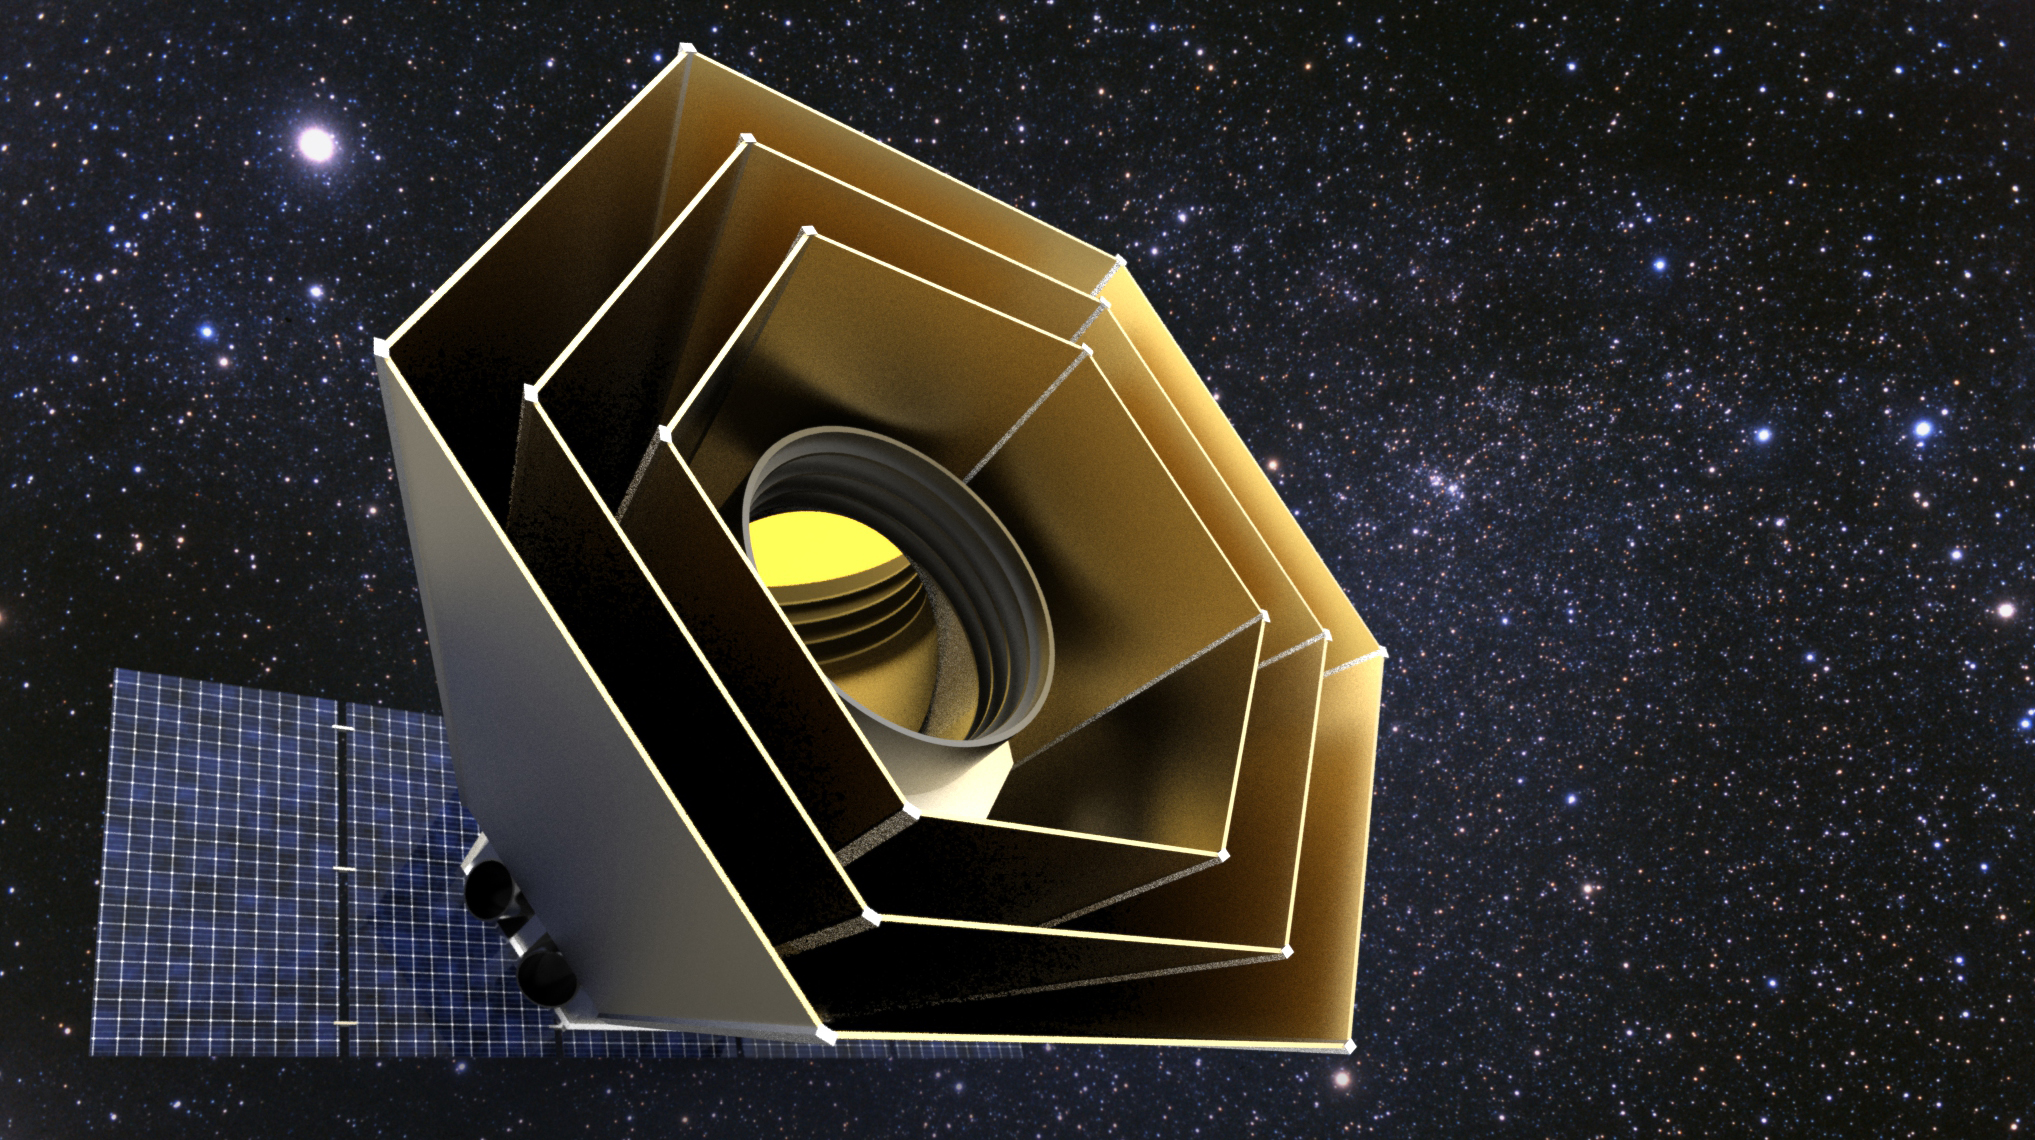
\includegraphics[width=.7\linewidth]{figs/cdim_cover-render.jpg}
  \caption{An artistic rendition of the Cosmic Dawn Intensity Mapper stationed at Sun-Earth \Ltwo.}
\label{fig:cover}
\end{figure}

The Cosmic Dawn Intensity Mapper (CDIM) is a concept for a Probe-class \SI{1.5}{\meter} aperture telescope, passively cooled to \SI{45}{\kelvin}, with an actively cooled $6\times6$ detector array that utilizes linear variable filters (LVFs)~\cite{cooray2016cdim2page} capable of three-dimensional spectro-imaging observations over the wavelength range of 0.75 to \SI{7.5}{\micro\meter} at a spectral resolving power R$=500$.
CDIM has a \SI{10}{\deg\squared} instantaneous field of view (FoV) atop a focal plane of thirty-six $2048\times2048$ detectors.
The survey strategy using spacecraft operations following a shift and stare mode will result in 1360 independent narrow-band spectral images of the sky on a given location.
Surveys are planned to span from \SI{25}{\deg\squared} up to \SI{1000}{\deg\squared} over a five year lifetime in an orbit about Sun-Earth Lagrange point L$_{2}$\@.

Although Wide Field Infrared Survey Telescope (WFIRST) will be capable of \SI{3400}{deg\squared} wide area surveys, its spectroscopy is limited to \SI{2}{\micro\meter}, limiting the selection of galaxies it is able to observe~\cite{wfirstFinal2012}.
While James Webb Space Telescope (JWST) is capable of targeted spectroscopy studies of galaxies present in reionization and surveys \SI{10}{armin\squared} for reionization galaxies~\cite{Gardner2006}, CDIM will make use of tomographic intensity mapping of spectral emission lines to study the aggregate statistical properties of the sources and their spatial distribution.
The intensity of the Ly$\alpha$ and H$\alpha$ lines, combined with others, will also provide critical clues to the formation of metals in the universe~\cite{cooray2016cdim2page}.

% What is a "Probe-class" mission?
Probe-class missions occupy a role on a larger scale than Discovery missions, such as Kepler and Dawn, but not as large as Flagship missions such as JWST.\@
Such missions are intended to be PI-led scientific investigations rather than general observatories, and have a firm \$1B cap~\cite{probeclasswp}.
Critical design requirements to achieve CDIM's science goals as a Probe-class mission are summarized in~\autoref{tab:critical-params}.
CDIM will leverage mature and flight-proven technology to reduce development costs.
% CDIM is optimized to search for the first cosmic sources of dust and evidence of the very earliest stellar populations, bridging the gaps in the JWST and WFIRST cosmic dawn surveys and exceeding them in capability.

\begin{table*}
  \caption{Critical design requirements for the CDIM spacecraft.}
  \small\centering
  \begin{tabular}{@{}llll@{}} \toprule
    Spacecraft Design Driver & Impact & Target \\ \midrule
    Cost & Science capability, instrument architecture & less than \$\SI{1}{B} \\
    Mass & Launch vehicle & less than \SI{1000}{\kilo\gram} \\
    Temperature (OTA) & Passive radiator & \SI{45}{\kelvin} \\
    Temperature (Detector) & Cryocooler & \SI{35}{\kelvin} \\
    Pointing Requirements & Attitude control system & less than \SI{0.5}{arcsec} \\
    Lifetime & Redundancy, RCS propellant & \SI{5}{years} \\
    Orbit & Solar array, thermal management, launch vehicle, telemetry & Sun-Earth \Ltwo{} \\
    \bottomrule
  \end{tabular}
\label{tab:critical-params}
\end{table*}

\section{Optical Telescope Assembly}
\label{sec:ota}
% \label{sec:mirror}
% Recall requirements such as FoV, spectral resolution. Technical requirement of temperature.
Preliminary explorations indicate that a $1.3$--$1.5$\si{\meter} aperture off-axis primary mirror cooled to \SI{45}{\kelvin} is required to meet CDIM's spectro-imaging  requirements~\cite{cooray2016cdim2page}.
The primary mirror is notionally assumed to be constructed from light-weighted Corning (ultra-low expansion) silica-titania glass with a honeycomb core and a gold-deposition surface coating.
For this type of mirror, the estimated mass is in the neighborhood of \SI{200}{\kilo\gram}.

% \subsection{Detectors}
% \label{subSec:detector}
For near-IR observations, the primary mirror must be cooled to cryogenic temperatures.
Rather than including a heating element and detectors that operate at warm temperatures, it is advantageous to use detectors that operate at cryogenic temperatures as well so as to minimize thermal radiation that could be detrimental to near-infrared (near-IR) observations.

A $6\times6$ array of $2048\times2048$ pixel detectors is required cover a \SI{10}{deg\squared} focal plane with \SI{1}{arcsec} pixels.
HgCdTe infrared detectors meet CDIM design goals of operating at cryogenic temperatures, low in cost, and, of course, sensitive in near-IR.\@
Several types of HgCdTe detectors satisfy CDIM's spatial resolution, wavelength range, and sensitivity requirements.
These detectors range in technology-readiness-level (TRL), but all are sufficiently developed to be considered for the 2020~Decadal and will be demonstrated on missions such as NEOCam, SPHEREx, and JWST~\cite{dore4872spherex,Gardner2006}.
Candidate detectors are listed in~\autoref{tab:detectors}.

\begin{table}[!h]
  \centering
  \caption{Candidate $2048\times2048$ pixel detectors for the CDIM FPA~\red{cite cdim proposal}.
\label{tab:detectors}}
  \begin{tabular}{@{}lccc@{}} \toprule
            & TRL & Wavelength Range          & Heritage \\ \midrule
    HyVisi  & 4   & 0.5--0.8\si{\micro\meter} & $1024\times1024$ (TRL 9) \\
    H2RG-2.5& 8   & 0.9--2.5\si{\micro\meter} & $1024\times1024$ (TRL 9) \\
    H2RG-5.0& 8   & 2.5--5.0\si{\micro\meter} & $1024\times1024$ (TRL 9) \\
    H2RG-8.0& 4   & 5.0--10.0\si{\micro\meter} & $1024\times1024$ (TRL 6) \\ \bottomrule
  \end{tabular}
\end{table}

CDIM will utilize 36 detectors in a close-packed, $6\times6$ mosaic focal plane assembly (FPA).
In the expected normal operating mode, each detector dissipates less than \SI{4}{\milli\watt}, for a total power dissipation of less than \SI{150}{\milli\watt} for the full array.

Linear-variable filters (LVFs) will be placed just above the detectors to provide spectral dispersion for spectrometry.
LVFs are simple, space-qualified solutions to permit spectral data cubes between $0.75$--$7.5$\si{\micro\meter} that are commercially available and significantly lower in cost than more complex systems~\cite{photonicsdotcom2016lvf}.

CDIM optics, instruments, and focal plane will be housed in an aluminum light-tight box that is be bead blasted to a matte finish and black anodized.
The purpose of this housing is to reduce reflections and scattered light from the exposed, reflective portions of the detectors.

The optical telescope assembly (OTA) as a whole is estimated to have a mass of 200--250\si{\kilo\gram}.

\section{Thermal Design}
\label{sec:thermal}
% General approach to cooling with passive and active. Explain tradeoffs between passive and active.
CDIM will employ both passive and active thermal regulation systems.
By using passive radiators in tandem with an active cryocooler, the static OTA heat load can be dissipated by the lightweight radiator and a smaller cryocooler may be used to only cool the detector array rather than the whole OTA mass plus FPA.\@
Passive cooling is used to cool the OTA and FPA from solar radiation, while active cooling regulates heat dissipated by active detectors.

The OTA is cooled to \SI{45}{\kelvin} to reduce background photon load in the near-IR.\@
Passive thermal regulation is maintained using a multi-stage V-groove radiator, which bounces radiative heat into the \SI{3}{\kelvin} background of space~\cite{bard_1987}.

\begin{figure}[!hb]
  \centering
  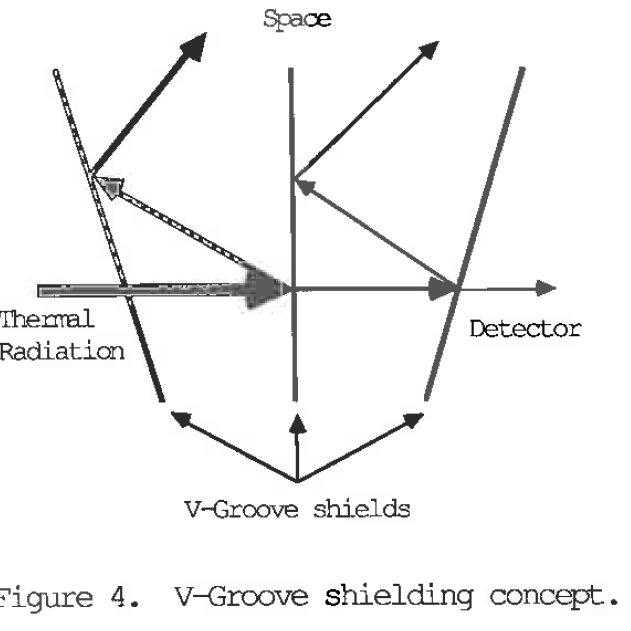
\includegraphics[width=.5\linewidth]{figs/vgroove-concept.png}
  \caption{Low emmissivity, high specular surface vanes are nested at a slight angle to reflect thermal radiation into space~\cite{rasbach1988}. \red{Replace this figure with a powerpoint graphic.}}
\label{fig:v-groove}
\end{figure}

V-groove radiators have been demonstrated in passive cryogenic radiators up to \SI{4}{\kelvin} with Planck, SPIRIT, and Spitzer (warm mission).\@
Like Planck, the active coolers are also pre-cooled to less than \SI{50}{\kelvin} this way~\cite{shinozaki2014spica}.
In order to achieve passive cooling from a baseline temperature of \SI{300}{\kelvin} at Sun-Earth Lagrange point \Ltwo, CDIM will feature a \red{\SI{x}{\meter\squared} $x$-stage} V-groove radiator.
\red{Since CDIM may be at various angles of incidence to solar radiation as it surveys the sky, the V-groove radiator fins will extend outward, more like SPHEREx than Planck}.

CDIM's thermal requirement to reduce thermal noise in the detector array can be met by actively cooling the array to \SI{35}{\kelvin} by a mechanical cryocooler.
Stirling-cycle mechanical refrigerators are low-vibration, high-reliability, and lightweight active cryocooling systems that have significant heritage in space applications.
Pulse-tube mechanical cryocoolers are similar to Stirling cryocoolers in capacity, cost, and function.
While Stirling cryocoolers use mechanisms to drive the thermodynamic cycle, Pulse-tube cryocoolers use an acoustic standing wave.
Either type of cryocooler is suitible for CDIM, and both types have significant heritage in space applications~\cite{gilmore2003spacecraft}.
One candidate system is Raytheon's PSC 1-stage Stirling cryocooler, capable of cooling a \SI{1.2}{\watt} parasitic heat load to \SI{35}{\kelvin}.
This cryocooler is \SI{18.6}{\kilo\gram} and requires \SI{88}{\watt} of input power~\cite{gilmore2003spacecraft}.

In this configuration, the most significant heat loads from the cooled section come from conduction through the OTA support structure, which isolates the cooled section from the warm spacecraft bus.
Only the mirror and detectors need to be cooled to cryogenic temperatures.
Electronics boards that control the FPA and instrumentation need not be cryocooled.
These warm electronics are housed in CDIM's spacecraft bus with other spacecraft systems.
Some components that require cooling below the temperature of the bus, but not so far as the FPA, may be placed between stages of the V-groove radiator.
A notional map of heat transfer is shown in~\autoref{fig:heat-map}.

\begin{figure}[!ht]
  \centering
  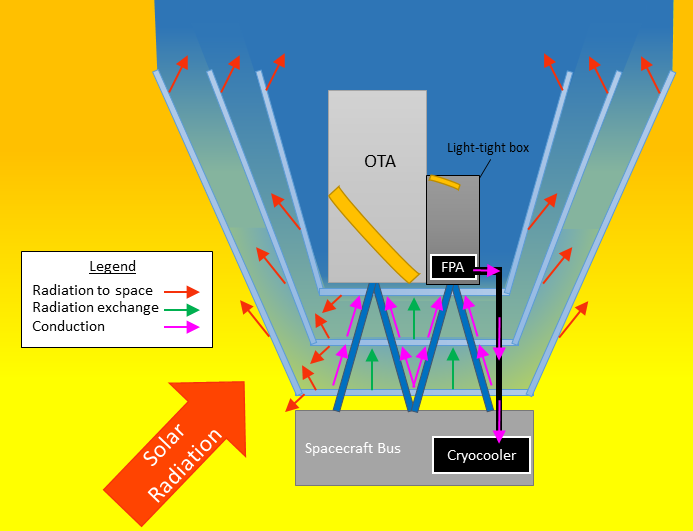
\includegraphics[width=.6\linewidth]{figs/heat-map.png}
  \caption{Notional pathways and heat loads throughout the cooled section are shown. Relative margnitude is indicated by arrow size.
\label{fig:heat-map}
}
\end{figure}

% Explain generally how v-groove radiators work.
% Used on planck and jwst.
% Desired final temp based on material, setup and location.
% Area based on general size of telescope.
% May need to be deployable, depending on required area.

% Detectors use active cooling to bring temp down to \SI{35}{\kelvin}.
% Explain why active needed to manage thermals of detectors.

% Describe types of cryocoolers and the high-level traits/tradeoffs between them. Choose one in particular, but leave wiggle room for others to be chosen.
% Explain the architecture for implementing this type of cooler, including power draw and mass.
% Active cooling will be achieved by a pulse-tube or stirling cycle mechanical cryocooler.

\section{Attitude Determination and Control}
\label{sec:adcs}
CDIM will be three-axis stabilized using an inertial reference unit and star-trackers.
Star trackers identify constellations in their field of view to determine the spacecraft's heading to within 1--3 arcseconds.
These systems are used to coarsely slew CDIM to a target.

Rather than using more accurate (and more expensive) inertial or star-tracking sensors, fine pointing guidance sensors may be included on the focal plane, as demonstrated by WFIRST~\cite{wfirstFinal2012}.
These fine guidance sensors enable CDIM to meet its relative pointing control requiremend of \SI{2.5}{arcsec}.
% Recall attitude control requirements for science objectives.
% To conduct a survey, the spacecraft must first understand its orientation and then act to align itself with a given area of the sky.
Redundant systems are included to allow CDIM to operate in different power states.
Low-fidelity attitude determination sensors such as sun sensors are cheap, accurate to less than one degree, and lightweight.
Sun sensors provide CDIM with a coarse safe-hold capability.
% Explain the star tracker among other attitude control systems. Select a class of star tracker.

% Briefly explain inertial and propulsive attitude control and the limitations of each.
In a heliocentric orbit, the primary disturbance to the spacecraft's heading is solar radiation pressure (SRP).
At \Ltwo, solar radiation pressure presents itself as torque on the spacecraft with a maximum load on the order of $10^{-5}$\si{\newton\meter}.

Hydrazine monopropellant thrusters will be used for orbit station-keeping as well as momentum management.
A desired heading is maintained by the spacecraft using a 3-axis zero-momentum inertial system, whereby the error in heading due to SRP is cancelled out by spinning up or slowing down reaction wheels.
Reaction wheel systems are capable of torques ranging from $.01$ to $1$\si{\newton\meter} and store $0.4$ to $3000$\si{\newton\meter\second} of practical momentum~\cite{smad2015}.
Power consumption varies with reaction wheel speed, with a maximum estimate of roughly \SI{100}{\watt}.
After some time the inertial attitude control may become saturated.
Desaturation is managed by engaging station-keeping thrusters for short periods of time.
Additionally, these thrusters will be used to maintain an orbit at \Ltwo{} as it is an inherently unstable orbit.

\section{Flight Computer}
% CDIM is capable of autonomous operation and system diagnostics.
\red{
  CDIM is capable of autonomous operation and system diagnostics.
  Nominal operation includes maintaining an attitude during imaging, capturing images, and downlinking data to Earth.
  Images will be processed on-board CDIM using an algorithm demonstrated by SPHEREx~\cite{spherexTelemetry2016}.
}

\section{Telemetry}
\label{sec:telemetry}
Typically for high-Earth and deep-space missions, the X-Band Space Science frequency band is used for uplink and downlink between the spacecraft and Ground Stations.
Thus, high-gain antennas are best suited for both links~\cite{smad2015}.

A survey conducted by CDIM will generate \red{\SI{168.39}{Gb}} of data per day employing on-board data processing akin to SPHEREx~\cite{spherexTelemetry2016}.
With a compression ratio of $2.5$:$1$, CDIM will downlink a total of \SI{63.7}{Gb/day} during a survey.
Transmission rates are dependent on the total time available for CDIM to send data to a ground station.
For example, the spacecraft could transmit continuously at a very low transfer rate, or send larger volumes of data once per day over 1 hour at the expense of a higher transfer rate.
\red{Example calculation of data to downlink 1 day in 1 hr.}

\begin{wstable}[htb]
  \caption{For redundancy, CDIM is outfitted with multiple communication modes.
  Downlink transfer rates reflect estitmates based on the target of \SI{63.7}{Gb/day}.
  Typical data transfer rates are outlined for uplinks~\cite{smad2015}.
\label{tab:telemetry}}
  \begin{tabular}{@{}lll@{}} \toprule
    Mode & Uplink & Downlink \\ \midrule
    Emergency & \SI{7.8}{bps} & $5$--$10$\si{bps} \\
    Engineering data & $15.6$--$2000$\si{kbps} & Up to \SI{10}{bps} \\
    Science data & $15.6$--$2000$\si{kbps} & \SI{0.74}{Mbps} (continuous) or \\
    & & \SI{17.7}{Mbps} (1 hour per day)\\\bottomrule
  \end{tabular}
\end{wstable}

Uplinks will follow standard protocols and do not require transmitting large volumes or particularly fast transfer rates.
The CDIM telemetry system, including antenna and power converter, are estimated to have a mass of \SI{2}{kg}.

\section{Power}
\label{sec:power}
Since CDIM will be located at \Ltwo, it is exposed to constant and significant solar flux.
All power generation will come from an array of photovoltaic cells facing the sun.
While the array may be fixed, the required area of the array is minimized if the cells are able to adjust to account for different incident angles to the sun.
The array will deploy after the launch and orbital insertion phases of the mission.

Based on a rough power budget and the spacecraft's position at \Ltwo, \red{the array must be min $x$--max $x$\si{\meter\squared}} in area to sustain operation.
The dark side of the array acts as a radiator to contribute to the thermal regulation of the spacecraft bus.

\red{Identify candidate systems.}

\section{Structure}
\label{sec:structure}
The mirror and detectors will be supported by low-moisture composites to provide adequate structure stiffness while minimizing mass and conductive heat loads to the cooled section.

The spacecraft bus will be a graphite epoxy composite hexagonal structure, which houses all non-instrumentation systems including the cryocooler, ADCS, telemetry, processing, power modules, and propulsion tank.
The bus will also provide hard points for integration with the launch vehicle.

%% WFIRST structure section
% the spacecraft bus is a
% graphite epoxy composite hexagonal structure, consisting
% of two modules (bus module and propulsion module)
% that house the spacecraft and payload electronics
% boxes and the propulsion tank. The spacecraft bus provides
% the interfaces to the payload and the launch vehicle
% and supports the Observatory launch mass of 2509
% kg, including margin (see Table 15). It supports a multipanel
% fixed solar array and a sunshield to prevent the
% Sun from illuminating payload hardware during science
% observations (see Figure 36). A

% \section{Mission Profile}
% \label{sec:mission-profile}
\section{Orbit}
\label{sec:orbit}
CDIM will orbit around Sun-Earth Lagrange point \Ltwo{} since it allows the spacecraft to be oriented such that half of the celestial sphere is visible at all times, and the spacecraft may oppose the Sun, Earth, and Moon concurrently and at all times.
This also leads to a very thermally stable environment.
\Ltwo{} is near enough to Earth (roughly 1.5 million \si{\kilo\meter}) so that CDIM may communicate with ground stations without the Deep Space Network, and maintains near-constant communications geometry~\cite{canalias2004}.

\begin{figure}[!h]
  \centering
  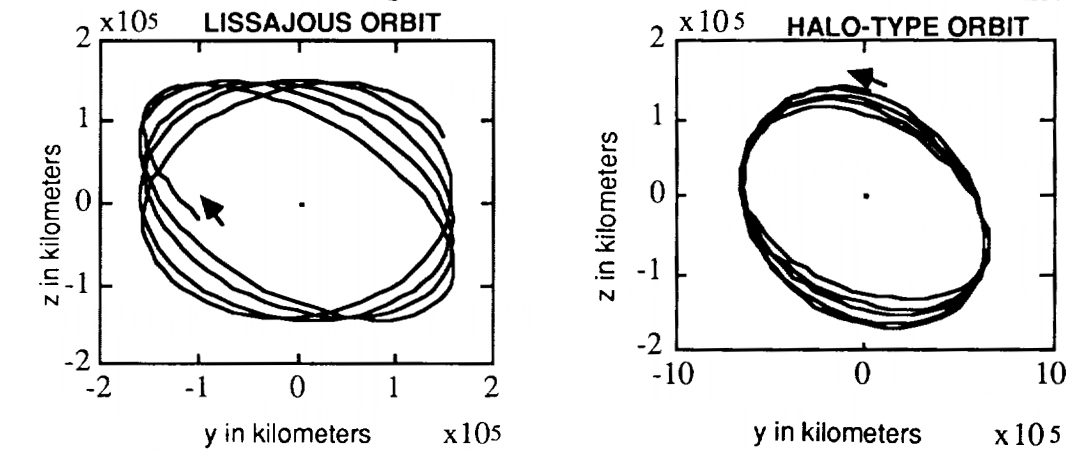
\includegraphics[width=.6\linewidth]{figs/orbits.png}
  \caption{
      \emph{Left:} Orthographic view of a quasi-periodic Lissajous orbit.
      \emph{Right:} Orthographic view of a periodic halo orbit.~\cite{gordon1993orbit}
\label{fig:orbits}
  }
\end{figure}

Around \Ltwo, two types of orbit are considered: Lissajous and halo-type orbits.
Lissajous orbits are quasi-periodic but may be smaller in radius than periodic halo orbits.
Halo orbits are more costly to achieve in terms of delta-v, or energy to transfer into such trajectory.
Station-keeping costs are not significantly different between the two orbits~\cite{gordon1993orbit}.
As such, CDIM may enter a Lissajous orbit around \Ltwo{} similar to the orbits of JWST and Herschel missions.

\section{Launch Vehicle}
\label{sec:launch}
CDIM will be comfortably within the mass and spatial limits of both currently available and development launch vehicles capable of delivering payloads to Sun-Earth Lagrange Point \Ltwo.
Future launch vehicles will be more than capable of delivering CDIM to \Ltwo, and industry trends indicate that heavy and super-heavy vehicles will continue to come online by the time CDIM launches.

Due to the rigorous launch environment, CDIM solar panels and passive radiators will not be deployed until CDIM is delivered to a transfer orbit en route to \Ltwo.

\begin{wstable}
  \caption{Available launch vehicle configurations and their capabilities to send NASA payloads to \Ltwo~\cite{rioux2016,spacelaunchreport}.
\label{tab:launch-vehicles}}
  \begin{tabular}{@{}lclr@{}} \toprule
    Vehicle & Payload to \Ltwo{} & Fairing size & Cost\tnote{$\dagger$} \\ \midrule
    Falcon 9 v1.1 & \SI{2900}{\kilo\gram} & $5.2\times13.1$ \si{\meter} & \$$97$\si{M}\\ \midrule
    Falcon Heavy\tnote{*} & \SI{14000}{\kilo\gram} & $5.2\times13.1$ \si{\meter} & \$$120$\si{M}\\ \midrule
    Atlas V 551 & \SI{6100}{\kilo\gram} & $4.2\times10.0$ \si{\meter} & \$$153$\si{M}\\
    & & $5.1\times11.0$ \si{\meter} & \\ \midrule
    Ariane V & \SI{6600}{\kilo\gram} & $5.4\times12.7$ \si{\meter} & \$$165$\si{M}\\
    & & $5.4\times13.8$ \si{\meter} & \\
    & & $5.4\times17.0$ \si{\meter} & \$$220$\si{M}\\ \midrule
    Delta IV Heavy & \SI{9800}{\kilo\gram} & $5.0\times14.3$ \si{\meter} & \$$375$\si{M}\\
    & & $5.0\times19.1$ \si{\meter} & \\ \bottomrule
  \end{tabular}
  \begin{tablenotes}
    \item{$\dagger$} Launch costs may be higher due to NASA mandated oversight and testing.
    \item[*] Costs and capacities are representative of design specifications for launch vehicles that are currently in development.
  \end{tablenotes}
\end{wstable}
%
% \subsection{Operations}
% \subsection{End of Life}



\section{Cost Estimation}
\label{sec:cost}
The overall cost of a space telescope may be broken down on the subsystem level.
All conclusions based on statistical analysis are only as good as their databases.
Fiscal data, such as what is required for proper analysis, is scarce.
Estimations are made with engineering judgement based on available data.

To estimate the cost of the CDIM mission, costs are separated into drivers of the \emph{mission cost}, which includes hardware, development, ground support, integration, testing, science, and management.
Existing generalized parametric cost estimation approaches identify key cost drivers for mission cost~\cite{stahl2013,bely2011}, but do not take labor or overhead costs into account.
Overhead and labor costs are included in a more robust model for \emph{total cost}, where:

\begin{equation}
  	\text{Total Cost}=(1.5)\times\text{Mission Cost}
\label{eq:total-cost}
\end{equation}

\citeauthor{stahl2013} present an approach to estimating OTA cost based on correlations with data on flown space telescope missions.
CDIM's projected costs may be obtained from these findings with engineering judgement, knowing that the data is drawn from a relatively small sample set.
Thus, an OTA aperture diameter of \SI{1.5}{\meter} yields a median OTA cost of \$58.2M.
Since OTA cost is found, estimates for other cost drivers may be obtained from relative cost values.
\begin{wstable}[htp]
  \centering
  \begin{tabular}{@{}lrrr@{}}\toprule
                          &                   & \multicolumn{2}{c}{Est. Cost} \\
    Driver                & \% Mission Cost   & \SI{1.3}{\meter} & \SI{1.5}{\meter} \\ \midrule
    OTA                   & \SI{13}{\percent} & \$48.0M & \$58.2M \\
    Spacecraft            & \SI{20}{\percent} & \$76.8M & \$91.3M \\
    Instruments           & \SI{15}{\percent} & \$57.6M & \$69.8M \\
    Ground Support        & \SI{5}{\percent}  & \$18.8M & \$22.8M \\
    Integration \& Testing & \SI{7}{\percent} & \$25.6M & \$31.0M \\
    Systems Engineering   & \SI{4}{\percent}  & \$16.0M & \$19.4M \\
    Management            & \SI{4}{\percent}  & \$16.0M & \$19.4M \\
    R\&D                  & \SI{21}{\percent} & \$80.0M & \$97.0M \\
    Science Team          & \SI{10}{\percent} & \$37.6M & \$45.6M \\ \midrule
    Mission Cost          &                   & \$188.2M & \$456.5M \\
    Labor \& Overhead     &                   & \$376.5M & \$228.2M \\
    Total Cost            &                   & \$564.7M & \$684.7M \\ \bottomrule
  \end{tabular}
  \caption{CDIM total cost breakdown by driver. \red{Make total cost less dependent on OTA cost. Ground support and science costs shouldnt rise so much along with OTA cost. Maybe just show one diameter and hide the other graph.}
\label{tab:total-cost}
}
\end{wstable}

\begin{figure}[!h]
    \centering
    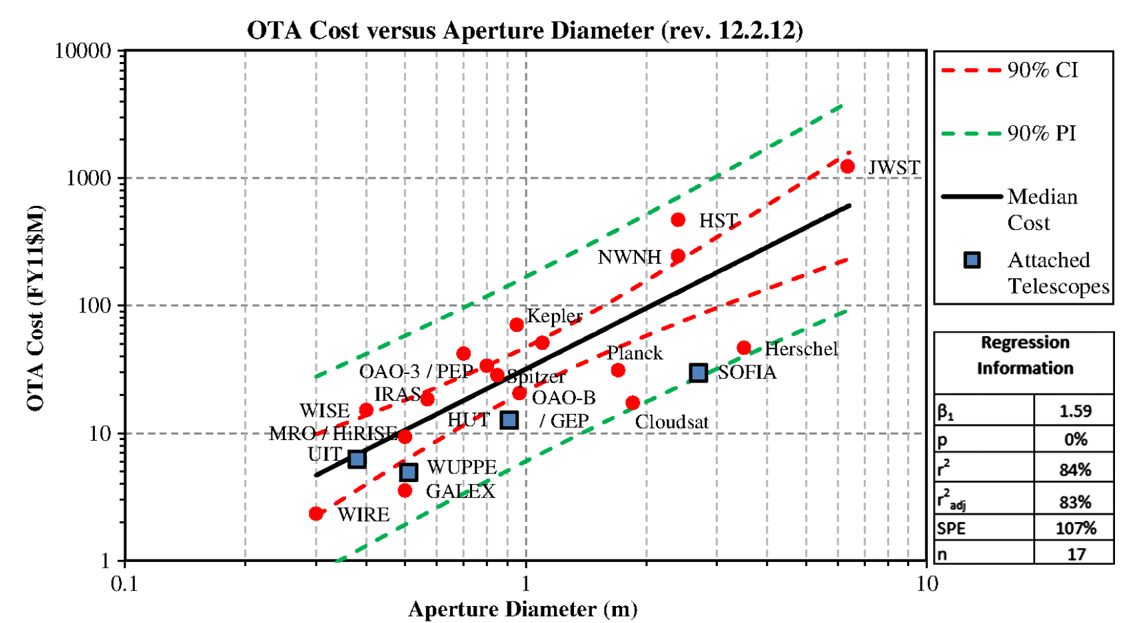
\includegraphics[width=.8\linewidth]{figs/ota_cost-diameter_stahl2010.png}
    \caption{Optical Telescope Assembly vs.\ cost correlation~\cite{stahl2013}. Given a target OTA aperture diameter of \SI{1.5}{\meter} for CDIM, a reasonable estimate of OTA cost is obtained from the median cost trendline.
\label{fig:cost-stahl-ota-cost-vs-diameter}
}
\end{figure}

\begin{figure}[!h]
  \centering
    \centering
    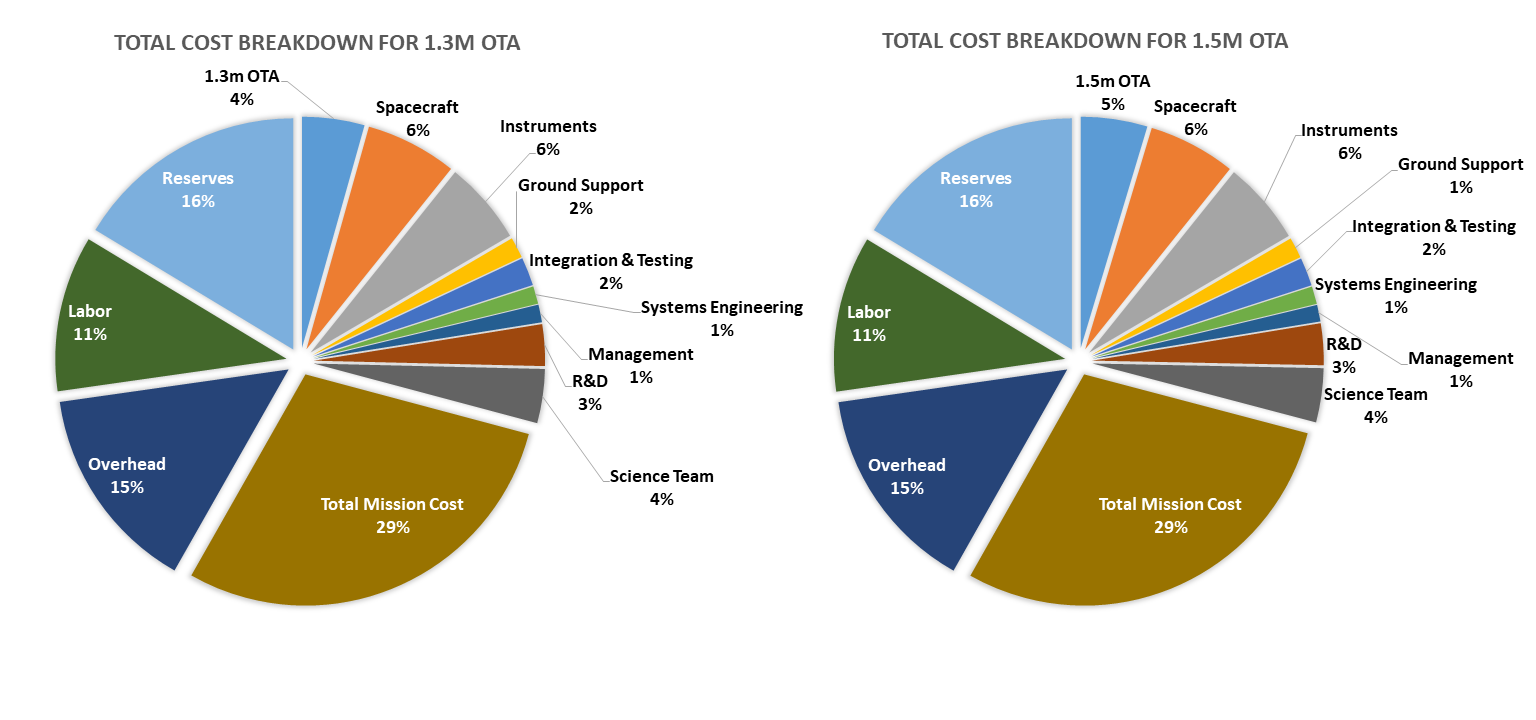
\includegraphics[width=.6\linewidth]{figs/cost-breakdown-pie.png}
    \caption{CDIM estimated cost breakdown in percent of mission cost.
\label{fig:cost-breakdown}
}
\end{figure}

% \begin{figure}[!h]
%   \centering
%   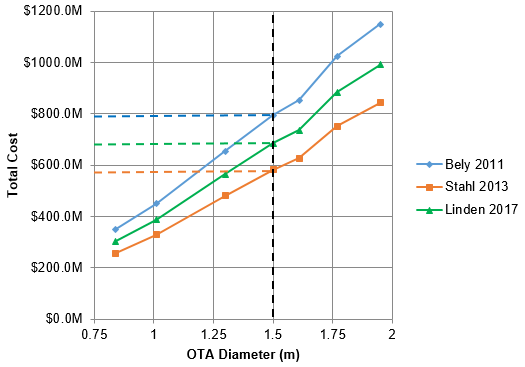
\includegraphics[width=.6\linewidth]{figs/total-cost-vs-diameter.png}
%   \caption{CDIM total cost relation to OTA aperture diameter under various cost models. The model described here is robust and presents a conservative estimate compared to similar models by \citeauthor{bely2011} and \citeauthor{stahl2013}, after a total cost approximation is applied following \autoref{eq:total-cost}.
% \label{fig:cost-total-compare-models}
% }
% \end{figure}

% The most robust model for the CDIM mission predicts its total cost to be \$684.7M, and even the more conservative model predicts CDIM costing to fall under \$800M.
The CDIM mission has significant margin under the \$1B cap for Probe-class missions.

\clearpage

\section{Conclusion}
\label{sec:conclusion}
% Summarize points made above. Notable points include mirror diameter, detector, power budget, mass budget, total cost, and the fact that technologies are already significantly developed.
\begin{figure}[htp]
  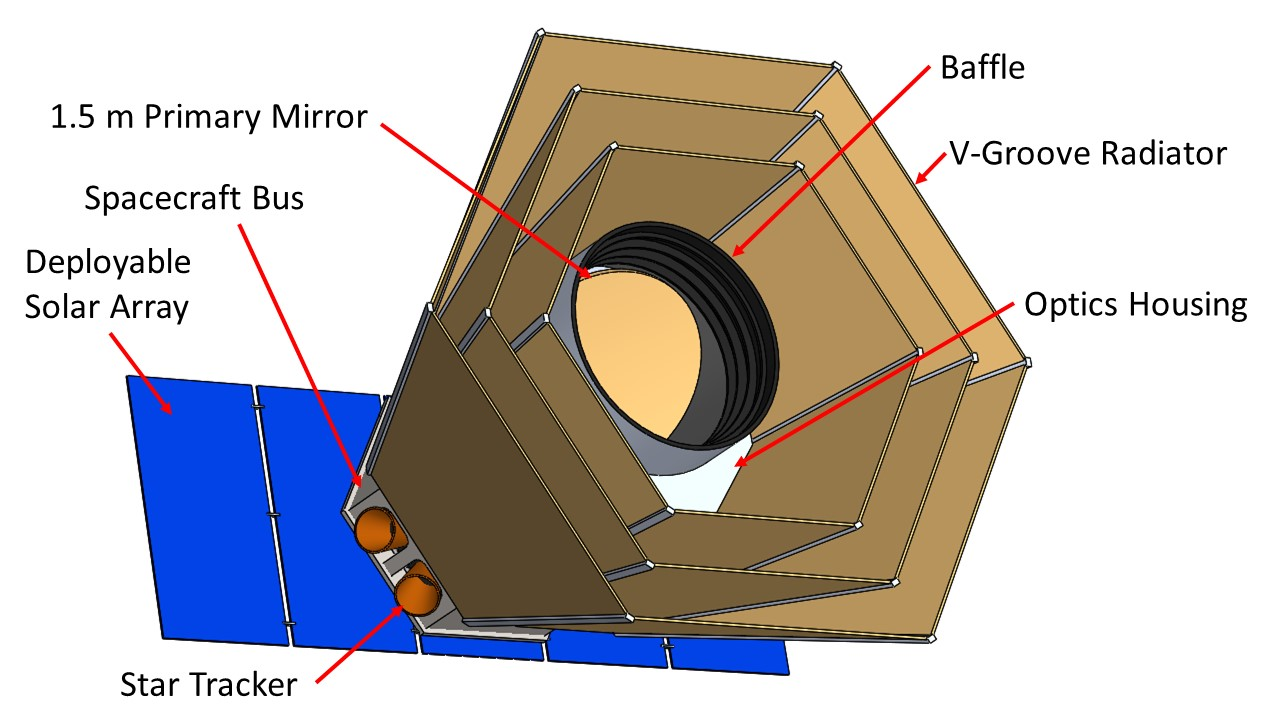
\includegraphics[width=\linewidth]{figs/cdim_annotated-cartoon}
  \caption{CDIM consists of a passively cooled \SI{1.5}{\meter} aperture OTA, actively cooled focal plane, and off-the-shelf spacecraft components where applicable. \red{Add cutaway view.}}
\label{fig:cdim-annotated}
\end{figure}
\section*{Acknowledgments}
Thanks.

\bibliography{cdim_design}

\end{document}
